\subsection*{Partie A}
\begin{enumerate}
	\item D'après l'énoncé voici l'arbre pondéré des évènements $F$ et $I$ :

	\begin{center}
	
	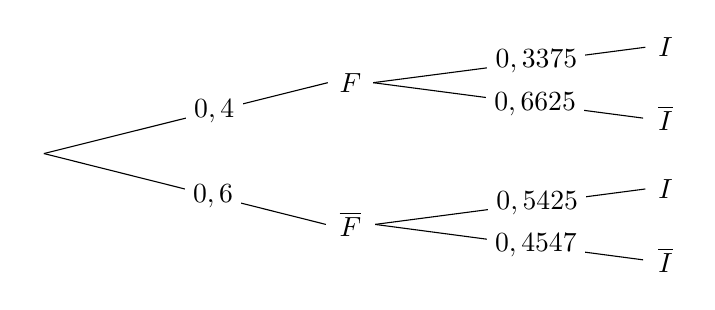
\begin{tikzpicture}[xscale=1,yscale=1,baseline={(R.base)}]
		
		\tikzstyle{noeud}=[fill=white,circle,inner sep=2pt]
		\tikzstyle{feuille}=[fill=white,circle,inner sep=2pt]
		\tikzstyle{etiquette}=[pos=0.6,fill=white, inner xsep=3pt, inner ysep=1.5pt]
		
		\def\DistanceInterNiveaux{4}
		\def\DistanceInterFeuilles{0.9}
		
		\def\NiveauA{(0)*\DistanceInterNiveaux}
		\def\NiveauB{(1)*\DistanceInterNiveaux}
		\def\NiveauC{(2)*\DistanceInterNiveaux}
		\def\InterFeuilles{(-1)*\DistanceInterFeuilles}
		
		\node[noeud] (R) at ({\NiveauA},{(1.5)*\InterFeuilles}) {};
		\node[noeud] (Ra) at ({\NiveauB},{(0.5)*\InterFeuilles}) {$F$};
		\node[feuille] (Raa) at ({\NiveauC},{(0)*\InterFeuilles}) {$I$};
		\node[feuille] (Rab) at ({\NiveauC},{(1)*\InterFeuilles}) {$\overline{I}$};
		\node[noeud] (Rb) at ({\NiveauB},{(2.5)*\InterFeuilles}) {$\overline{F}$};
		\node[feuille] (Rba) at ({\NiveauC},{(2)*\InterFeuilles}) {$I$};
		\node[feuille] (Rbb) at ({\NiveauC},{(3)*\InterFeuilles}) {$\overline{I}$};
		
		\draw (R.east)--(Ra.west) node[etiquette] {$0,4$};
		\draw (Ra.east)--(Raa.west) node[etiquette] {$\np{0,3375}$};
		\draw (Ra.east)--(Rab.west) node[etiquette] {$\np{0,6625}$};
		\draw (R.east)--(Rb.west) node[etiquette] {$\np{0,6}$};
		\draw (Rb.east)--(Rba.west) node[etiquette] {$\np{0,5425}$};
		\draw (Rb.east)--(Rbb.west) node[etiquette] {$\np{0,4547}$};
	\end{tikzpicture}
	
	














	\end{center}

	\item Il faut trouver $P(F \cap I)=  P(F) \times P_F(I) = 0,4 \times \np{0,3375} = 0,135$.

	\item On a de même $P\left(\overline{F} \cap I\right)=  P\left(\overline{F}\right) \times P_{\overline{F}}(I) = 0,6 \times \np{0,5425} = \np{0,3225}$.

	D'après la loi des probabilités totale la probabilité que l'élève choisi au hasard envisage des études d'ingénieur est égale à :

	$P(I) = P(F \cap I) + P\left(\overline{F} \cap I\right) = 0,135 + \np{0,3225} = \np{0,4605}$.

	\item On calcule $P_I(F) = \dfrac{P(F \cap I)}{P(I)} = \dfrac{0,135}{\np{0,4605}} \approx \np{0,2932}$ soit $0,293$ au millième près.

	Parmi les élèves envisageant des études d'ingénieur un peu moins de 30\,\% sont des filles.
\end{enumerate}

\subsection*{Partie B}
\begin{enumerate} \item
	\begin{enumerate}
		\item Le nombre $n$ est assez grand pour que l'on puisse considérer que chaque fille choisie ait une probabilité de vouloir devenir ingénieure est égale à 0,15 : la variable $X$ suit donc une loi binomiale de paramètres $n$ et $p = 0,15$.

		\item On sait que $E  = n \times p = n \times 0,15 = 0,15n$.
	\end{enumerate}
	\item On a : $P(X \geqslant 1) = 1 - P(X = 0) =\ds 1 - \binom{n}{0} \times 0,15^0 \times (1 - 0,15)^n = 1 - 0,85^n$.

	Il faut donc que $P(X \geqslant 1) \geqslant 0,99 \iff 1 - 0,85^n \geqslant 0,99 \iff 0,01 \geqslant 0,85^n$,

	d'où par croissance de la fonction logarithme népérien :

	$\ln 0,01 \geqslant n\ln 0,85 \iff \dfrac{\ln 0,01}{\ln 0,85} \leqslant n$ car $\ln 0,85 < 0$.

	Or $\dfrac{\ln 0,01}{\ln 0,85} \approx 28,3$.

	Il faut donc interroger au moins 29 lycéennes.

	\item On a $\dfrac{29}{4} = 7,25$. Il faut donc choisir sur les 29 filles 8 qui souhaitent devenir ingénieure, d'où :

	$P(X\geqslant 8) = 1 - P(X < 8) = 1 - P(X \leqslant 7)
	$ : la calculatrice donne environ $0,059$ : sur 29 filles interrogées la probabilité qu'au moins le quart souhaite devenir ingénieure est légèrement inférieure à 6\,\%.
\end{enumerate}

\subsection*{Partie C}
\begin{enumerate}
	\item $S$ représente le nombre de lycéennes souhaitant devenir ingénieure parmi les \np{15000} lycéennes interrogées.

	\item $\mathrm{E}(S) = \mathrm{E}(X_1 + \ldots + X_{10}) = \mathrm{E}(X_1) + \ldots \mathrm{E}(X_{10})$ par linéarité ;

	$\mathrm{E}(S) = 10\mathrm{E}(X) $ car toutes les variables aléatoires ont la même espérance, donc :

	$\mathrm{E}(S) = 10 \times 225 = \np{2250}$.

	Il en est de même pour la variance de $S$ :

	$\mathrm{V}(S) = \mathrm{V}(X_1 + \ldots + X_{10}) = \mathrm{V}(X_1) + \ldots + \mathrm{V}(X_{10})$ car les lois sont indépendantes.

	$\mathrm{V}(S) = 10\mathrm{V}(X)$ car elles suivent la, même loi de probabilité.

	$\mathrm{V}(S) = 10 \times 191,25 = \np{1912,5}$.

	\item On sait que $S$ a une espérance. Utilisons l'inégalité de Bienaymé-Tchebychev pour minorer la probabilité  d'avoir un nombre de lycéennes désirant devenir ingénieure compris entre \np{2000} et \np{2500} :

	$P(\np{2000} < S < \np{2500})  = P(- 250 <S - \mathrm{E}(S) < 250) = P(|S - \mathrm{E}(S)| < 250)$ ou

	$P(\np{2000} < S < \np{2500})  = 1 - P(|S - \mathrm{E}(S)| \geqslant 250$ ;
	d'après l'inégalité de Bienaymé-Tchebychev :

	$P(\np{2000} < S < \np{2500}) \geqslant 1 - \dfrac{\mathrm{V}(S)}{250^2}$ soit

	$P(\np{2000} < S < \np{2500}) \geqslant 1 - \dfrac{\np{1912,5}}{\np{62500}}$

	$P(\np{2000} < S < \np{2500}) \geqslant 1 - \np{0,0306}$ et finalement,

	$P(\np{2000} < S <\np{2500}) \geqslant \np{0,9694} > 0,95$.

	Conclusion : à 5\,\% près l'affirmation est vraie.

\end{enumerate}
